\chapter{背景介绍}

模型检测将待检测的系统建模为一个跃迁系统(transition system),在时序逻辑(temporal logic)中指定待验证的属性。给定模型\(M\) 和属性\(\varphi\),模型检测将验证是否\(M\)满足\(\varphi\)。在不同的模型检测方法中,高级符号模型检查(Advanced Symbolic Model Checking)\citep{Grobelna_2015}使用简化的有序二叉决策图(Reduced Ordered Binary Decision Diagrams,ROBDDs 或 BDDs)\citep{Bryant_1986}来表示状态集合和转移关系。通过迭代调用图像计算算法来计算所有可达状态,判断一个模型是否满足时间属性,直到达到不动点为止。

最近,随着量子计算的发展,关于量子线路的验证技术也在不断发展\citep{viamontes2007checking,burgholzer2020advanced}。其中,利用模型检测方法对线路进行自动化验证也有了一些应用。由于量子线路运算空间随着量子比特的线性增加而指数级膨胀,传统的计算方法并不能很好应对。因此本文工作希望应用基于张量网络(tensor network)的张量决策图(tensor decision diagrams)进行量子模型检测。

而在本章中将简要介绍本文工作中的一些重要的基础知识。因此本章分为两节。第一节介绍量子计算相关背景,包括量子力学和量子线路。第二节介绍模型检测相关背景,包括跃迁系统,时序逻辑和量子模型检测。
\section{量子计算简介}
量子计算机(quantum computer)是一种利用量子比特特性进行计算的一种设备。在量子计算中,量子比特的特殊性质允许其同时处于多种状态,这与经典比特的二进制状态不同。量子计算机的状态空间可以用希尔伯特空间(Hilbert space)\(\mathcal{H}\)表示\citep{nielsen2010quantum},即可以进行内积运算(inner product)的复向量空间。比特状态可以用\(\mathcal{H}\)的向量表示,量子门由\(\mathcal{H}\)上的酉算子(unitary operator)表示。

量子线路(quantum circuit)是一种描述量子计算的模型。在量子线路中,通过量子比特的初始化、应用量子门、测量以及其他可能的操作的序列来构建和执行量子计算任务。量子线路通常从左向右阅读,每个量子门的作用是将输入的量子比特状态转变为输出状态,该过程可以认为是量子门的酉矩阵与输入的量子状态的乘积。
\begin{example}
    \label{ex-epr}
    图\ref{fig:example_cir} 所示的量子线路展示了一个具体的量子线路示例,可以用于制备EPR态。其中有单比特门\(H=\frac{1}{\sqrt2}\left[\begin{matrix}1&1\\1&-1\\\end{matrix}\right]\),以及双比特门\(CX=\left[\begin{matrix}\begin{matrix}1&0\\0&1\\\end{matrix}&\begin{matrix}0&0\\0&0\\\end{matrix}\\\begin{matrix}0&0\\0&0\\\end{matrix}&\begin{matrix}0&1\\1&0\\\end{matrix}\\\end{matrix}\right]\)。假设该量子线路的初始状态为\(\left|\psi\right\rangle=\left|0\right\rangle\left|0\right\rangle\),则输出状态为:
\begin{align}
   CX\cdot H\otimes I \cdot \left|\psi\right\rangle = \frac{|00\rangle+|11\rangle}{\sqrt{2}}
\end{align}
具体计算过程将在\ref{sec-cir}节中介绍。
\end{example}
\begin{figure}[!htbp]
    \centering
    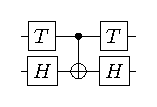
\includegraphics[width=.4\textwidth]{Img/example_cir.pdf}
    \caption{制备EPR态的量子线路图}
    \label{fig:example_cir}
\end{figure}



在量子计算机上可以执行各种算法和计算任务,如量子搜索\citep{Grover_1996}、量子因子分解\citep{Shor}和量子模拟\citep{Feynman}等。量子计算的潜力在于其能够在某些特定问题上比经典计算机更高效地进行计算,尤其在处理大规模数据和解决复杂问题方面具有潜在优势。本节对该部分进行简单介绍,而需要对这部分深入了解的读者,可以自行阅读
\citep{nielsen2010quantum}。
\subsection{量子力学}
量子力学有两种主要的表述:波动力学和矩阵力学。其中波动力学由Erwin Schrödinger首创,矩阵力学由Werner Heisenberg首创。波动力学使用微分方程为数学基础,更接近于经典物理的波动理论,适用于处理时间演化问题和连续系统。
而矩阵力学使用线性代数为数学基础,适用于具有离散能级的系统。由于在量子计算中,大量使用矩阵力学作为理论基础。
因此本小节主要介绍矩阵力学。
\subsubsection*{线性代数}
线性代数的基本研究对象是向量空间(vector space),也称作线性空间(Linear Spaces)。这是一种抽象的数学结构,用于描述向量的集合。向量空间在向量加法(Vector Addition)和标量乘法(scalar multiplication)封闭。
对于一个向量空间,向量的类型满足特定条件。向量可以是几何向量、函数、多项式或任何满足向量空间公理的对象。
同时还需要定义标量域(Scalars)\(\mathbb{F}\) ,在大多数情况下,标量是实数(Real Numbers)\(\mathbb{R}\)或复数(Complex Numbers)\(\mathbb{C}\),用于通过标量乘法运算改变向量的大小。
最后向量空间的还需要遵循一系列公理。这些公理规定了向量加法和标量乘法的性质,如加法的交换律和结合律、加法和标量乘法的分配律、加法单位元的存在性(即零向量,Zero Vector),以及乘法单位元(即标量1)的存在性。这些公理确保了向量空间内运算的一致性和预测性。

此外子空间(Subspace)也是是向量空间中的一个重要概念。子空间指的是一个向量空间的一个子集,同时它自身也是一个向量空间。因此子空间遵循向量空间的向量加法和标量乘法运算封闭的性质。线性算子 (Linear Operator),也称为线性映射(Linear Mapping)或线性变换(Linear Transformation),是在向量空间中的一种特殊函数,它在两个向量空间之间映射向量,保持向量加法和标量乘法的结构。% 线性算子定义
设 \(V\) 和 \(W\) 是两个向量空间,一个线性算子 \(T: V \rightarrow W\) 必须满足以下两个条件:
\begin{enumerate}
    \item 加法性 (Additivity):对于所有 \(u, v \in V\),有 \(T(u + v) = T(u) + T(v)\)。
    \item 齐次性 (Homogeneity):对于所有标量 \(a \in \mathbb{F}\) 和所有 \(v \in V\),有 \(T(av) = aT(v)\)。
\end{enumerate}
当$T$是\(T: W \rightarrow W\)的线性算子,则$T$是定义在向量空间$W$上的线性算子。其中恒等算子(identity operator)$T$是向量空间$W$上的线性算子,满足以下条件:
\begin{align}
    T(w) = w,\forall w \in W
\end{align}

此外有的向量空间还有内积和张量积(Tensor product)操作。内积定义为:\(( \cdot, \cdot ): V \times V \rightarrow \mathbb{F}\),其中 $V$ 是一个向量空间。对于任意两个向量 $u$ 和 $v$,它们的内积 $( u, v )$ 满足以下性质:
\begin{enumerate}
    \item 共轭对称性(Conjugate Symmetry): \(( u, v ) = \overline{( v, u )}\),其中\(\overline{( v, u )}\)是\(( v, u )\)的复共轭,当标量域为实数时,表现为对称性,即\(( u, v ) = ( v, u )\)。
    \item 线性 (Linearity)或齐次性:\(( \alpha u_1 + \beta u_2, v ) = \alpha( u_1, v ) + \beta( u_2, v )\),其中\(\alpha,\beta\in\mathbb{F}\)。
    \item 正定性 (Positive Definiteness):\(( v, v ) \geq 0\)且仅当\(v \)为加法单位元时等号成立。
\end{enumerate}
% 张量积定义
可以看到内积是一种特殊形式的线性算子。当两个向量内积为$0$时,称这两个向量正交。而张量积则提供了一种方法来构造新的向量空间。
设 \(V\) 和 \(W\) 是两个向量空间,它们的张量积 \(V \otimes W\) 是一个新的向量空间,满足以下性质:
\begin{enumerate}
    \item 对于每一对元素 \(v \in V\) 和 \(w \in W\),存在一个元素 \(v \otimes w \in V \otimes W\),称为它们的张量积。
    \item 张量积满足双线性性(Bilinearity):对于所有 \(v,v' \in V\),\(w,w' \in W\) 以及所有标量 \(a,b \in \mathbb{F}\),有
    \[
    (av + bv') \otimes w = a(v \otimes w) + b(v' \otimes w),
    \]
    \[
    v \otimes (aw + bw') = a(v \otimes w) + b(v \otimes w').
    \]
    \item 张量积是唯一的,意味着对于任何与 \(V \otimes W\) 具有相同性质的向量空间,都存在一个自然同构映射(Natural Isomorphism)到 \(V \otimes W\)。
\end{enumerate}

矩阵力学的数学基础建立在希尔伯特空间\(\mathcal{H}\),即一个可以进行内积运算的复向量空间。
希尔伯特空间中的向量由复数\(n\)元组\(\left(c_1,c_2,\cdots,c_n\right)\)构成,可以记作\(\mathbb{C}^n\),其中\(c\)表示复数。向量也可以有以下列矩阵形式:
\begin{align}
    \left[\begin{matrix}
        c_1\\c_2\\\vdots\\c_n
    \end{matrix}\right]
\end{align}
\(\mathbb{C}^n\)中的标量为复数。因此可以定义\(\mathbb{C}^n\)矩阵形式的标量乘法运算为:
\begin{align}
    c'\left[\begin{matrix}
        c_1\\c_2\\\vdots\\c_n
    \end{matrix}\right]=\left[\begin{matrix}
        c'\cdot c_1\\c'\cdot c_2\\\vdots\\c'\cdot c_n
    \end{matrix}\right]
\end{align}
其中等式右边的乘法为复数乘法,因此复数1为乘法单位元。类似地,\(\mathbb{C}^n\)矩阵形式的向量加法可以定义为:
\begin{align}
    \left[\begin{matrix}
        c_1\\c_2\\\vdots\\c_n
    \end{matrix}\right]
    +\left[\begin{matrix}
        c'_1\\c'_2\\\vdots\\c'_n
    \end{matrix}\right]=\left[\begin{matrix}
        c_1+c'_1\\c_2+c'_2\\\vdots\\c_n+c'_n
    \end{matrix}\right]
\end{align}
其中等式右边的乘法为复数加法,因此零向量的矩阵形式如下:
\begin{align}
    \left[\begin{matrix}
        0\\0\\\vdots\\0
    \end{matrix}\right]
\end{align}
通常将该向量记作\(\mathbf{0}\)。

类似地,可以定义\(\mathbb{C}^n\)矩阵形式的内积和张量积运算为:
\begin{align}
    \left(\left[\begin{matrix}
        c_1\\c_2\\\vdots\\c_n
    \end{matrix}\right]
    ,\left[\begin{matrix}
        c'_1\\c'_2\\\vdots\\c'_n
    \end{matrix}\right]\right)=
    \sum_{i=1}^{n}c_i^* c'_i
\end{align}
\begin{align}
    \left[\begin{matrix}
        c_1\\c_2\\\vdots\\c_n
    \end{matrix}\right]
    \otimes\left[\begin{matrix}
        c'_1\\c'_2\\\vdots\\c'_n
    \end{matrix}\right]=\left[\begin{matrix}
        c_1c'_1\\c_1c'_2\\\vdots\\c_1c'_n\\c_2c'_1\\\vdots\\c_n c'_n
    \end{matrix}\right]
\end{align}
在量子计算中,通常将向量\(\psi\)记作狄拉克右矢符号\(|\psi\rangle\)。
对向量\(|\psi\rangle\)中的复数全部取共轭,可以得到\(|\psi\rangle\)的共轭记作\(|\psi\rangle^*\)。
向量\(|\psi\rangle\)的共轭转置可以记作\(|\psi\rangle^\dagger\),也称对偶向量,可以用狄拉克左矢符号\(\langle\psi|\)表示。因此向量之间的内积也可以用以下方法表示:
\begin{align}
    (|\psi\rangle, |\phi\rangle)=\langle \psi|\phi\rangle , \forall |\psi \rangle, |\phi \rangle\in \mathcal{H}
\end{align}

希尔伯特空间\(\mathcal{H}\)中的线性算子集合,通常记作\(\mathcal{L} (\mathcal{H})\)。
对算子\(A \in \mathcal{L}\),$A$的伴随算子(adjoint operator)$A^\dagger$定义为:
\begin{align}
    \langle \psi |A^\dagger|\phi \rangle = \langle \phi |A|\psi \rangle^*, \forall |\psi \rangle, |\phi \rangle\in \mathcal{H}
\end{align}
算子\(A \in \mathcal{L}\),被称为作Hermite算子(Hermite operator),或者Hermitian,当且仅当满足以下条件:
\begin{align}
    A = A^\dagger
\end{align}


如果一个Hermitian算子\(A\)同时满足:
\begin{align}
    A^2 = A
\end{align}
那么\(A\)也被称作投影算子(project oroperator)。

如果一个Hermitian算子\(A\)同时满足:
\begin{align}
    A^\dagger A = A A^\dagger
\end{align}
那么\(A\)也被称作正规算子(normal oroperator)。同时\(A\)是正规算子,当且仅当被如下对角化:
\begin{align}
    A = \sum_{i}\lambda_i |i\rangle\langle i|
\end{align}
其中$\lambda_i$是$A$的特征值,$|i\rangle$为对应特征值的特征向量。

如果一个Hermitian算子\(A\)同时满足:
\begin{align}
    A^\dagger A = I
\end{align}
其中$I$表示希尔伯特空间中的恒等算子。那么\(A\)也被称作酉算子(unitary oroperator)。
酉算子保持向量之间的内积,即:
\begin{align}
    (U|\psi\rangle, U|\phi\rangle) = \langle \psi|U^\dagger U|\phi\rangle = \langle \psi|I|\phi\rangle = \langle \psi|\phi\rangle = (|\psi\rangle, |\phi\rangle), \forall |\psi \rangle, |\phi \rangle\in \mathcal{H}
\end{align}
\subsubsection*{量子力学基本假设}
在量子力学中,有四条基本假设,其数学框架是在不断实验中总结,假设,验证而得到的。
下面分别简单介绍一下这四条假设。
\begin{theorem}
    每个孤立的物理系统都可以通过一个内积复向量空间(即希尔伯特空间)来表征,此空间被视为系统的状态空间(state space)。该系统的全部性质由位于状态空间内的一个单位向量,即状态向量(state vector),完整定义。
\end{theorem}

量子力学的第一条假设,提出了量子系统的描述方式。最简单的量子系统是单个量子比特(qubit)构成的二维空间。
取$|0\rangle$和$|1\rangle$为该状态空间的一组标准正交基,则该状态空间中的所有状态向量$|\psi\rangle$都可以用以下方式表示:
\begin{align}
    |\psi\rangle = \alpha|0\rangle + \beta|1\rangle
\end{align}
其中$\alpha,\beta\in \mathbb{C}$,并满足:
\begin{align}
    |\alpha|^2+|\beta|^2  = 1
    \label{eq-cal}
\end{align}
等式\ref{eq-cal}确保了$|\psi\rangle$的模长为1,即保证了$|\psi\rangle$是单位向量:
\begin{align}
    \langle\psi|\psi\rangle = 1
    \label{eq-norm}
\end{align}
等式\ref{eq-norm}称为状态向量的归一化条件(normalization condition)。
而\(\alpha,\beta\)也被称为对应基状态向量的振幅(amplitude)。
该叠加态:
\begin{align}
    \frac{|0\rangle-|1\rangle}{\sqrt{2}}
\end{align}
处在$|0\rangle$状态的振幅为$\frac{1}{\sqrt{2}}$,处在$|1\rangle$状态的振幅为$-\frac{1}{\sqrt{2}}$。
\begin{theorem}
    一个封闭量子系统(closed quantum system)的演化(evolution)由酉变化(unitary operation)体现。具体来讲,系统在$t_1$时刻的状态$|\psi\rangle$与在$t_2$时刻的状态$|\psi'\rangle$之间,通过一个只与$t_1$和$t_2$两个时间点相关的酉操作符$U$连接:
    \begin{align}
        |\psi'\rangle = U|\psi\rangle
    \end{align}
\end{theorem}
酉变化可以用酉算子进行表示。对于酉算子$U$, 始终满足
\begin{align}
    U U^\dagger = I
\end{align}
这是因为这些演化都是可逆的。当令单个量子比特的状态空间的正交基$|0\rangle$和$|1\rangle$的矩阵形式为:
\begin{align}
    |0\rangle = \left[\begin{matrix}
        1\\0
    \end{matrix}\right],|1\rangle = \left[\begin{matrix}
        0\\1
    \end{matrix}\right]
\end{align}
可以得到常见单比特酉变化的矩阵形式,比如Pauli算子:
\begin{align}
    I = \left[\begin{matrix}
        1,0\\0,1
    \end{matrix}\right]
    \quad
    X = \left[\begin{matrix}
        0,1\\1,0
    \end{matrix}\right]
    \quad
    Y = \left[\begin{matrix}
        0,-i\\i,0
    \end{matrix}\right]
    \quad
    Z = \left[\begin{matrix}
        1,0\\0,-1
    \end{matrix}\right]
    \label{eq-pauli}
\end{align}
比如Hardmard算子和T门(也可以称为\(\pi/8\)门):
\begin{align}
    H = \frac{1}{\sqrt{2}}\left[\begin{matrix}
        1,1\\1,-1
    \end{matrix}\right]
    \label{eq-hardmard}
\end{align}
\begin{align}
    T = \left[\begin{matrix}
        1,&0\\0,&\exp(i\pi/4)
    \end{matrix}\right]
    \label{eq-t}
\end{align}

\begin{theorem}
    量子测量(quantum measurement) 可以通过一系列测量算子 (measurement operator) ${M_m}$ 刻画。这些算符作用于被测量系统的状态空间上。其中下标$m$
   对应实验中可能发生的测量结果。
\end{theorem}
由于测量结果的概率和为1,因此测量算子${M_m}$满足完备性,即:
\begin{align}
    \sum_m M_m\dagger M_m = I
\end{align}
假设测量前量子系统的状态为\(|\psi\rangle\),那么测量后得到结果m的概率为
\begin{align}
    p(m) = \langle\psi|M_m^\dagger M_m|\psi\rangle
\end{align}
测量后,系统的状态变为
\begin{align}
    |\psi'\rangle =  \frac{M_m|\psi\rangle}{\sqrt{p(m)}} = \frac{M_m|\psi\rangle}{\langle\psi|M_m^\dagger M_m|\psi\rangle}
\end{align}
\begin{theorem}
    复合系统(composite system) 的状态空间是其各个子空间的状态空间的
    张量积。如果复合系统从$1$到$n$的子系统,并且第$i$个系统的状态为$|\psi_i\rangle$。则复合系统的状态为\(|\psi_1\rangle\otimes|\psi_2\rangle\otimes\cdots\otimes |\psi_n\rangle\)。
    \label{th-com}
\end{theorem}
假设\ref{th-com}中的复合系统,假设了子系统之间的相互作用,并没有改变复合系统状态空间的结构。
此时的复合系统处于直积状态(product state)。例如两个处于\(|0\rangle\)状态的单量子组成的双量子比特的复合系统,可以有以下方式的表示:
\begin{align}
    |0\rangle\otimes|0\rangle=\left[\begin{matrix}
        1\\0
    \end{matrix}\right]\otimes\left[\begin{matrix}
        1\\0
    \end{matrix}\right] = \left[\begin{matrix}
        1\\0\\0\\0
    \end{matrix}\right]
\end{align}
此外还存在复合系统的量子状态不能分解成各个子系统量子状态的张量积的情况。此时复合系统处于纠缠状态(entangled state),复合系统不能表示为子系统的张量积形式。
例如该双量子比特的复合系统的状态,就不能表示为任何单比特状态向量的张量积:
\begin{align}
    \frac{|00\rangle+|11\rangle}{\sqrt{2}}
\end{align}
\subsection{量子线路}
\label{sec-cir}
在计算机中,通常使用图灵机作为抽象模型。
在讨论图灵机时,通常会设想一个容量无限的计算机。然而在实际中,计算机的容量是有限的。
因此在实际中,一般会使用一种替代的计算模型,线路模型。该模型在计算力方面与图灵机相当,但在许多应用场景中更为实用和符合实际。线路是由导线(wire)和逻辑门(gate)构成,它们分别负责信息的传递和基本计算操作。
\begin{example}
    图\ref{fig-not}展示了一个简单的经典线路。它以单个比特作为输入。这个比特通过一个门,该门会翻转比特,将1变为0,将0变为1。门前后的导线仅用于将比特信息传输到非门并从非门传出。
\begin{figure}[htbp]
    \centering
    \includegraphics[width=.3\textwidth]{Img/Not-gate-en}
    \caption{执行单个非门的经典基本线路}
    \label{fig-not}
\end{figure}
\end{example}

在量子计算中,一般使用量子线路(quantum curcuit) 作为抽象模型。
在量子线路中,逻辑门为量子操作,导线则传递量子比特信息。量子操作可以由量子门(quantum gate) 表示。
根据量子门作用的量子比特数,量子门可以被分为单量子比特门(single qubite gate)和多量子比特门(multiple qubit gate)。多量子比特门中比较常见的是双量子比特门。
以受控门(controlled gate)为例,其
输入量子比特分别为控制量子比特(control qubit)和目标量子比特(target qubit)。
假设$U $是作用于目标量子比特的任意单比特量子操作,则称该门为受控$U$门。
受控$U$门根据控制量子比特的值,决定是否将量子操作$U$作用于目标量子比特。
若控制量子比特的值为\(|0\rangle\),则目标量子比特值\(|\psi\rangle\)不变,若控制量子比特的值为
\(|1\rangle\), 则目标量子比特值变为\(U|\psi\rangle\)。

和经典线路模型不同,量子线路的量子信息一般从左到右传递。量子线路模型也可以看作经过一系列量子门,将线路左边的输入量子状态转换为线路右边的输出量子状态的模型。
因此通过量子线路可以描述各种量子进程。
\begin{example}
    单量子比特门Hadamard门为例,其矩阵形式为式子\ref{eq-hardmard}。因此其将输入的\(|0\rangle\)状态变换为
\(\frac{|0\rangle+|1\rangle}{\sqrt{2}}\)状态,\(|1\rangle\)状态变换为\(\frac{|0\rangle-|1\rangle}{\sqrt{2}}\)状态。其量子线路符号表示如图\ref{fig-h}所示。
\begin{figure}[htbp]
    \centering
    \includegraphics[width=.3\textwidth]{Img/hardmard-gate.pdf}
    \caption{Hadamard门的量子线路符号}
    \label{fig-h}
\end{figure}

    而受控门中最常见的是受控非门(controlled not gate),其矩阵形式为式子\ref{eq-cx}。
    \begin{align}
        \label{eq-cx}
        CX=\left[\begin{matrix}
            1 & 0 & 0 & 0\\
            0 & 1 & 0 & 0\\
            0 & 0 & 0 & 1\\
            0 & 0 & 1 & 0\\
        \end{matrix}\right]
    \end{align}
    因此若控制量子比特为\(|0\rangle\)则不做变换;若为\(|1\rangle\)则对目标量子比特进行比特翻转,将
输入的\(|0\rangle\)变换为\(|1\rangle\),\(|1\rangle\)变换为\(|0\rangle\)。其量子线路符号如图\ref{fig-cx}。
\begin{figure}[htbp]
    \centering
    \includegraphics[width=.3\textwidth]{Img/cnot-gate.pdf}
    \caption{受控非门的量子线路符号}
    \label{fig-cx}
\end{figure}

综上,例子\ref{ex-epr}中,包含一个Hadamard门和一个受控非门的制备EPR态的量子线路。当输入态为\(|00\rangle\)时,输出态为\(\frac{|00\rangle+|11\rangle}{\sqrt{2}}\)。具体计算过程如式子\ref{eq-eqr-cal}所示。
\begin{equation}
    \label{eq-eqr-cal}
    \begin{aligned}
        |\psi_{out}\rangle &=  CX\cdot H\otimes I \cdot \left|\psi_{in}\right\rangle\\
        &= CX\cdot H\otimes I \cdot \left|00\right\rangle\\
        &= CX\cdot H\otimes I \cdot \left|0\right\rangle\otimes \left|0\right\rangle\\
        &= CX\cdot H\left|0\right\rangle\otimes I\left|0\right\rangle\\
        &= CX\cdot \frac{|0\rangle+|1\rangle}{\sqrt{2}} \otimes\left|0\right\rangle\\
        &= \frac{|0\rangle|0\rangle+|1\rangle\otimes X|0\rangle}{\sqrt{2}}\\
        &=\frac{|00\rangle+|11\rangle}{\sqrt{2}}
    \end{aligned}
\end{equation}
\end{example}
\section{模型检测简介}
本节将简要介绍了模型检测中的跃迁系统、时序逻辑的验证以及量子模型检测。跃迁系统是模型检测的基础,定义了系统状态、行为及状态转移关系。时序逻辑用于指定待验证的属性,包括状态命题和路径命题。而量子模型检测利用Birkhoff-von Neumann量子逻辑描述量子系统的性质,展示了量子逻辑中命题的表示和逻辑结构。这些都为本文工作的研究提供了重要的理论基础。
\subsection{跃迁系统}
\label{sec-transition}
跃迁系统广泛应用于模型检测中待检测系统的建模,其定义为\citep{baier2008principles}:
\begin{equation}
\mathcal{M}=(S, S_0, \Sigma, R)
\end{equation}
其中\(S\)为系统状态集合,\(S_0\)为系统初态集合,因此满足\(S_0\subseteq S\)。 $\Sigma=\{\sigma_1,\ldots,\sigma_m\}$ 表示符号的集合,而 $R \subseteq S \times \Sigma \times S$ 则代表转移关系。此外还有\(AP\)为描述系统原子命题。L是标记函数,将状态映射为状态满足的原子命题集合。需要验证的属性\(\varphi\)将表述为命题。对于某个状态集 $S' \subseteq S$,通过转移关系 $R$ 得到的系统状态可以表示为
\begin{equation}\label{eq:image}
R(S') := { t\in S \mid (s, \sigma, t) \in R\ \text{并且}\ s \in S', \sigma \in \Sigma}.
\end{equation}


系统的有限路径片段\(\pi\)是一个有限状态序列\(s_0,s_1\ldots s_n\),其中\(s_0\in S_0\)。\(s_i\)满足\(s_{i-1}\overset{\sigma_i}{\rightarrow}s_i,\sigma_i\in \Sigma\),对于所有\(0<i\leq n\),其中\(n\geq 0 \)。无限路径片段\(\pi\)是一个无限状态序列\(s_0,s_1\ldots\),使得对于所有\(i>0\),\(s_{i-1} \overset{\sigma_i}{\rightarrow}  s_i,\sigma_i\in \Sigma\)。在路径中\(\pi\left[i\right]=s_i,\pi\left[i\right)=s_i\ldots\)。所有以\(S_0\)为开始的路径,构成了路径集合\(Path\left(S_0\right)\)。

量子模型检测的跃迁系统类似。区别在于状态空间用\(\mathcal{H}\),转移关系为量子操作。一个量子自动机定义如下:
\begin{align}
    \mathcal{M}=\{\mathcal{H},S,\Sigma,\mathcal{T}\}
\end{align}
\begin{example}
    
    图\ref{fig:transition-system} 所示的跃迁系统展示了一个简化版的售货机模型。在该模型中,用户投入硬币,进行选择后就可以得到苏打水或者啤酒。在该例子中,系统状态\(S=\{pay,select,soda,beer\}\),系统初态\(S_0=pay\)。
    系统行为\(\Sigma=\{insert\_coin,\tau,get\_soda\),\\\(get\_beer\}\),其中\(\tau\)表示立即行动符号。转移关系图中已经展示。原子命题可取\(AP=\{paid,drink\}\)。因此\(L\left( pay \right)=\{\varnothing\}\),\(L\left(soda\right)=L\left(beer\right)=\{paid,drink\}\),\(L\left(select\right)=\{paid\}\)。系统的一个路径是\(\pi=pay\ select\ soda\ pay\ selsect\ \ldots\)。此时\(\pi\left[1\right]=slect,\pi\left[1\right)=select\quad soda\quad pay\quad selsect\ldots\)。同时该路径满足\(\pi\in Path\left(pay\right)\)。
    \begin{figure}[!htbp]
        \centering
        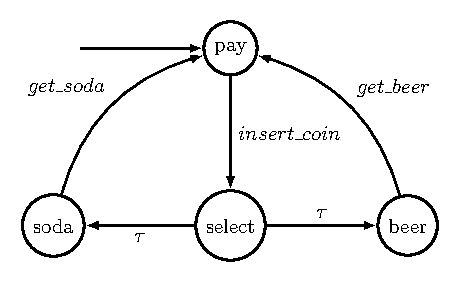
\includegraphics[width=.6\textwidth]{Img/map.pdf}
        \caption{一种简化版的售货机跃迁系统}
        \label{fig:transition-system}
    \end{figure}
\end{example}

\subsection{时序逻辑中的可达性问题}
本小节将简单介绍时序逻辑中的可达性问题。在量子模型检测中,与经典模型检测一样使用时序逻辑指定待验证的属性\(\varphi\)。时序逻辑命题的运算符有两类\citep{goranko_2023}。状态命题公式(State formulas):\(\varphi ::=a\left|\exists\varphi\right|\forall \varphi\left|\lnot\varphi\right|\varphi\land\psi\),其中\(a\in AP\)。以及路径命题公式(Path formulas):\(\varphi\Colon=O\varphi|\varphi U\psi\)。给定模型的一个状态为\(s\),路径为\(\pi\),则具体满足条件分别如下:
\begin{itemize}
    \item \(s\models a,iff \L\left(s\right)\models a\)
    \item \(s\models\exists\varphi,iff\ \pi\models\varphi\)对一些\(\pi\in Path\left(s\right)\)
    \item \(s\models\forall\varphi,iff\ \pi\models\varphi\)对所有\(π\in Paths\)
    \item \(s\models\lnot\varphi,iff\ s\nvDash\varphi\)
    \item \(s\models\varphi\land\psi,iff\ s\models\varphi\ and\ s\models\psi\)
    \item \(\pi\models O\varphi,iff\ \pi\left[1\right]\models\varphi\)
    \item \(\pi\models\varphi U\psi,iff\ \exists j\geq0\).\(\pi\left[j\right)\models\psi\) 同时对所有\(0\le i<j\)有\(\pi\left[i\right)\models\varphi\)
\end{itemize}


图\ref{fig:path-formula-basic} 展示了两种路径命题公式的直观示意图。


\begin{figure}[!htbp]
    \centering
    \begin{subfigure}[b]{0.8\textwidth}
        \centering
        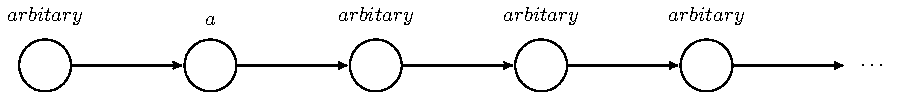
\includegraphics[width=\textwidth]{Img/path_for_Oa.pdf}
    \end{subfigure}
    \\
    \begin{subfigure}{0.8\textwidth}
        \centering
        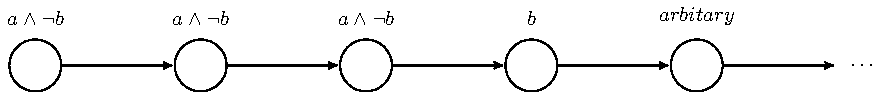
\includegraphics[width=\textwidth]{Img/path_for_aUb.pdf}
    \end{subfigure}
    \caption{路径命题公式$\pi\models O a $与 $\pi\models a U b$的图示}
    \label{fig:path-formula-basic}
\end{figure}
在模型检测中,有三类比较重要的可达性问题,分别是可达性、持续可达性以及重复可达性。过程中主要涉及以下路径命题公式:\(\lozenge\) 表示最终(eventually),\(\square\)表示总是(always),\(\lozenge\square\)表示总是最终(always eventually),\(\square\lozenge\)表示最终总是(eventually always)。其中\(\lozenge\)和\(\square\)具体定义为:
\begin{itemize}
    \item \(\lozenge\varphi\overset{\text{def} }{=} \text{True}U\varphi\)
    \item \(\square\varphi\overset{\text{def} }{=} \neg\lozenge\neg\varphi\)
\end{itemize}
图\ref{fig:path-formula}展示了这两种基本路径命题公式的直观示意图。
\begin{figure}[!htbp]
    \centering
    \begin{subfigure}[b]{0.8\textwidth}
        \centering
        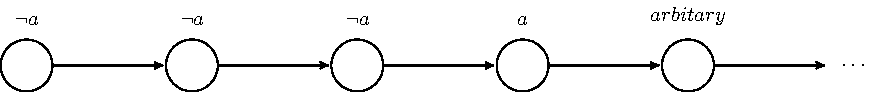
\includegraphics[width=\textwidth]{Img/path_for_Dia.pdf}
    \end{subfigure}
    \\
    \begin{subfigure}{0.8\textwidth}
        \centering
        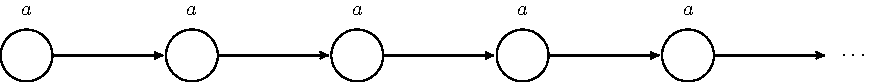
\includegraphics[width=\textwidth]{Img/path_for_SQa.pdf}
    \end{subfigure}
    \caption{路径命题公式$\pi\models\lozenge a$与 $\pi\models\square a$的图示}
    \label{fig:path-formula}
\end{figure}

具体的可满足条件为:
\begin{itemize}
    \item \(\pi\models\lozenge\varphi,iff\exists j\ge0.\pi[j)\models\varphi\)
    \item \(\pi\models\square\varphi,iff\forall j\ge 0.\pi[j)\models\varphi\)
    \item \(\pi\models\lozenge\square\varphi,iff\exists i\ge 0.\forall j\ge i,\pi[j)\models\varphi\)
    \item \(\pi\models\square\lozenge\varphi,iff\forall i\ge 0.\exists j\ge i,\pi[j)\models\varphi\)
\end{itemize}
基于此三种可达性问题定义分别如下:
\begin{itemize}
    \item 可达性:\( Pr^{\mathcal{M}}(s \models \lozenge G) = Pr^M(\pi \models \lozenge G : \pi \in \text{Paths}(s))\)
    \item 持续可达性:\( Pr^{\mathcal{M}}(s \models \lozenge \square G) = Pr^M(\pi \models \lozenge \square G : \pi \in \text{Paths}(s))\)
    \item 重复可达性:\( Pr^{\mathcal{M}}(s \models\square \lozenge G) = Pr^M(\pi \models \square\lozenge G : \pi \in \text{Paths}(s))\)
\end{itemize}
\begin{example}
    根据上文的路径命题公式和满足条件,可以解释下列命题:
    \begin{itemize}
        \item $\square\lozenge\varphi$: 对于每一个时间点 \(i\),都存在某个时间点 \(j \geq i\) 使得 \(\varphi\) 在时间点 \(j\) 为真;即\(\varphi\) 无限次地成立。
        \item $\lozenge\square\varphi$: 存在一个时间点 \(i\) 使得 \(\varphi\) 从 \(i\) 开始在所有时间点 \(j \geq i\) 时为真;即\(\varphi\) 最终永远成立。
        \item $\square(\text{请求} \rightarrow \lozenge\text{响应})$: 每一个请求最终都会得到响应。
      \end{itemize}
\end{example}
\subsection{量子模型检测}
目前量子的模型检测,主要使用Birkhoff-von Neumann Quantum Logic来描述量子系统的性质\citep{birkhoff1987logic}。Birkhoff-von Neumann量子逻辑是一种非经典逻辑,用于描述量子力学中事件的逻辑结构。它由 Birkhoff 和 von Neumann 在 1936 年首次提出。在量子逻辑中,命题的集合不再形成布尔代数,而是形成一个投影算子的正交完备格,这与传统的逻辑系统不同。而需要对本小节深入了解的读者,可以自行阅读\citep{2021}。

\subsubsection*{量子命题}
\label{sec-logic}
在 Birkhoff-von Neumann 量子逻辑中,量子系统的状态可以由希尔伯特空间(Hilbert space)来描述,每个量子命题对应希尔伯特空间的一个闭子空间。对于系统的状态 \(|\psi\rangle\),如果它属于某个特定的闭子空间 \( \mathcal{X} \),可以说这个命题是真的。

\begin{example}
    考虑以下量子逻辑命题:

\begin{itemize}
\item 命题 \( \mathcal{X} \):在时间 \( t \) 时,量子粒子的位置 \( x \) 坐标在区间 \( [a, b] \) 内。
\item 命题 \( \mathcal{Y} \):在时间 \( t \) 时,量子粒子的动量 \( y \) 坐标在区间 \( [a, b] \) 内。
\end{itemize}
这些命题 \( \mathcal{X} \) 和 \( \mathcal{Y} \) 可以通过粒子的状态希尔伯特空间的特定子空间来表示。
\end{example}


上述将子空间视为原子命题的想法也可以用量子测量来解释。假设系统的一个基本性质由希尔伯特空间$\mathcal{H}$的一个闭子空间$\mathcal{X}$描述。
在量子力学中,为了检查这个性质是否满足,需要对系统当前态$|\psi\rangle$执行一个二元(是或否)测量$\{P_{\mathcal{X}}, P_{\mathcal{X}}^{\perp}\}$,
其中$P_{\mathcal{X}}$和$P_{\mathcal{X}}^\perp$分别是到$\mathcal{X}$和它的正交补$\mathcal{X}^\perp$的投影。测量结果通常是非确定性,其对应概率分别为:
\begin{itemize}
    \item $\mathcal{X}$在$|\psi\rangle$中满足的概率是$\langle\psi|P_{\mathcal{X}}|\psi\rangle$。
    \item 不满足的概率是
    $\langle\psi|P_{\mathcal{X}}^\perp|\psi\rangle = 1 - \langle\psi|P_{\mathcal{X}}|\psi\rangle$。
\end{itemize}
同时可以通过设置一个阈值$\lambda \in [0,1]$来定义关于满足的概率的量化关系:

\begin{definition}
    如果$\langle\psi|P_{\mathcal{X}}|\psi\rangle \rhd \lambda$,则称$|\psi\rangle$是$(\lambda, \rhd)$满足子空间$\mathcal{X}$描述的命题。其中其中$\rhd \in \{<, \leq, >, \geq\}$。 
\end{definition}

在本文工作的研究中只考虑定性满足,即阈值$\lambda$为0或1时的$(\lambda, \rhd)$满足。显然,对于任何纯态$|\psi\rangle$和子空间$\mathcal{X}$,都有:

\begin{itemize}
\item 如果$|\psi\rangle \in \mathcal{X}$,那么$\mathcal{X}$在$|\psi\rangle$中$(1, \geq)$-满足;
\item 如果$|\psi\rangle \in \mathcal{X}^\perp$,那么$\mathcal{X}$在$|\psi\rangle$中$(0, \leq)$-满足。
\end{itemize}

\subsubsection*{量子逻辑中的连接词}
\label{sec-connect}
在数学上,这种集合的命题逻辑结构可以使用格理论(lattice theory)来描述,其中格中的元素对应于量子事件,格的操作则对应于逻辑运算。在确定了原子命题后,需要引入连接词,这些连接词可以用来构建更复杂的命题,以描述量子系统的复杂属性。在语义上,这些可以被视为在希尔伯特空间$\mathcal{H}$的一个子空间 \(S(\mathcal{H})\) 中的代数操作。
具体如下:

\begin{itemize}
    \item 子空间之间的包含关系 \( \subseteq \) 在 \(S(\mathcal{H})\) 中是一个偏序关系,它可以理解为量子逻辑的蕴含(元逻辑)。
    \item 一个子空间 \( \mathcal{X} \) 的正交补 \( \mathcal{X}^\perp \) 在量子逻辑中用作否定的解释。
    \item \(S(\mathcal{H})\) 对交集是封闭的,即对于 \(S(\mathcal{H})\) 中的任何元素族 \( \{\mathcal{X}_i\} \),都有$\bigcap_{i} \mathcal{X}_{i} \in \mathcal{S}(\mathcal{H})$。在量子逻辑中用于表示合取。
    \item 对于一组子空间 \(\{\mathcal{X}_i\}\),这些子空间的并定义为
    \(
    \bigvee_i \mathcal{X}_i = \text{span} \left( \bigcup_i \mathcal{X}_i \right).
    \)。在量子逻辑中,析取被解释为子空间的并。
\end{itemize}


量子逻辑中的析取被解释为子空间的并运算。\( (S(\mathcal{H}), \cap, \vee, \perp) \) 构成一个正交模格(orthomodular lattice),\( \subseteq \) 是其序关系,这是 Birkhoff–von Neumann 量子逻辑的代数模型。

在实际应用中,通常只选择$\mathcal{S}(\mathcal{H})$的一个子集$AP$作为原子命题的集合。$AP$的元素可以被看作是真正关注的命题,而其他命题可能是无关的。为了算法的目的,通常假设$AP$是$\mathcal{S}(\mathcal{H})$的一个可列或者甚至是有限的子集,而不是作为原子命题的集合使用$\mathcal{S}(\mathcal{H})$本身,因为$\mathcal{S}(\mathcal{H})$是无穷无尽的。

\subsubsection*{量子逻辑中的满足}
在量子逻辑中,“满足”(satisfaction)意味着量子系统的状态可以在逻辑表达式指定的条件下被视为真。对于任何原子命题$\mathcal{X} \in AP$和状态$|\psi\rangle \in \mathcal{H}$,如果$|\psi\rangle \in \mathcal{X}$,那么说状态$|\psi\rangle$满足$\mathcal{X}$。用$L(|\psi\rangle)$表示在状态$|\psi\rangle$中被满足的原子命题集合:

\begin{equation}
L(|\psi\rangle) = {\mathcal{X} \in AP : |\psi\rangle \in \mathcal{X}}.
\end{equation}

有时,需要在一个状态$|\psi\rangle$和一个不在$AP$中的命题$\mathcal{X}$之间建立更一般的满足关系。例如,在某些应用中,可能对一个命题$\mathcal{X}$是否被一个状态$|\psi\rangle$满足感兴趣,但由于内存的考虑,量子模型检测中一般只会选择了一个非常有限的不包括$\mathcal{X}$的原子命题集合。

对于这样一个不在$AP$中的命题$\mathcal{X}$。给定一个原子命题集合$AP$,其中$\mathcal{X} \in \mathcal{S}(\mathcal{H})$。
如果$\bigcap_{\mathcal{Y} \in L(|\psi\rangle) }\mathcal{Y} \subseteq \mathcal{X}$,那么状态$|\psi\rangle$满足$\mathcal{X}$,记作$|\psi\rangle \models_{AP} \mathcal{X}$或简单地$|\psi\rangle \models \mathcal{X}$。
直观地说,$\bigcap_{\mathcal{Y} \in L(|\psi\rangle)} \mathcal{Y}$是可以用原子命题来定义并描述状态$|\psi\rangle$的最弱陈述。因此,包含关系意味着在状态$|\psi\rangle$中成立的原子命题集合共同蕴含命题$\mathcal{X}$。而如果$\mathcal{X} \in AP$,那么$|\psi\rangle \models \mathcal{X}$当且仅当$|\psi\rangle \in \mathcal{X}$。

\begin{example}
    设$\mathcal{H}$是一个$n$维希尔伯特空间,它的标准正规基是$\{|0\rangle, |1\rangle, \cdots, |n - 1\rangle\}\ (n \geq 2)$,令$|\psi\rangle = \frac{1}{\sqrt{2}}(|0\rangle + |1\rangle)$。
    \begin{itemize}
        \item 如果取$AP$为与基态$|0\rangle$正交的子空间:

        \begin{equation}
        AP = {\mathcal{Y} \in \mathcal{S}(\mathcal{H}) : |0\rangle \perp \mathcal{Y}},
        \end{equation}
        
        那么$L(|\psi\rangle) = \varnothing$,因此
        
        \begin{equation}
        {\bigcap_{\mathcal{Y} \in L(|\psi\rangle)} \mathcal{Y} = \mathcal{H}.}
        \end{equation}
        
        所以对于任何$\mathcal{X} \in \mathcal{S}(\mathcal{H})$,有$|\psi\rangle \models \mathcal{X}$当且仅当$\mathcal{X} = \mathcal{H}$。
        
        \item 设$AP$为$\mathcal{H}$的2维子空间。对于$n = 2$的情况,
        \begin{equation}
            {\bigcap_{\mathcal{Y} \in L(|\psi\rangle)} \mathcal{Y} = \mathcal{H}}
            \end{equation}
            
            那么有$|\psi\rangle \models \mathcal{X}$当且仅当$\mathcal{X} = \mathcal{H}$。对于$n > 2$的情况,
            
            \begin{equation}
            {\bigcap_{\mathcal{Y} \in L(|\psi\rangle)} \mathcal{Y} = \operatorname{span}\{|\psi\rangle}\}
            \end{equation}
            
            并且$|\psi\rangle \models \mathcal{X}$当且仅当$|\psi\rangle \in \mathcal{X}$。
            
        \item 如果$AP$是包含基态$|2\rangle$的子空间,即$AP = \{\mathcal{X} \in \mathcal{S}(\mathcal{H}) : |2\rangle \in \mathcal{X}\}$,那么
            
            \begin{equation}
            {\bigcap_{\mathcal{Y} \in L(|\psi\rangle)} \mathcal{Y} = \operatorname{span}\{|\psi\rangle, |2\rangle}\}
            \end{equation}
            
            并且$|\psi\rangle \models \mathcal{X}$当且仅当$|\psi\rangle,|2\rangle \in \mathcal{X}$。
    \end{itemize}

\end{example}
\section{本章小结}
本章主要介绍了本文工作的研究的相关背景知识,包括量子计算和模型检测的基础理论。

第一部分介绍了量子计算的相关知识,包括量子力学基本原理、量子线路模型等。量子力学建立在希尔伯特空间、算符等数学基础之上,描述了量子系统的状态、演化和测量。量子线路则是一种描述量子计算的模型,通过对量子比特进行初始化、施加量子门操作和测量等来执行量子计算任务。

第二部分介绍了模型检测的基础知识,包括跃迁系统、时序逻辑和量子模型检测。跃迁系统用于对待检测系统建模,定义了系统状态、行为及状态转移关系。时序逻辑用于指定待验证的属性,讨论了状态命题和路径命题等。量子模型检测则利用Birkhoff-von Neumann量子逻辑描述量子系统的性质,阐述了量子逻辑中命题的表示、逻辑结构及满足关系等。

本章的背景知识为后续开展基于TDD的量子模型检测研究奠定了理论基础。
% 本章最后指出,通过张量网络表示量子线路和量子系统,并借助张量决策图进行量子模型检测是本文工作的研究的主要目标。

% 总的来说,本章对量子计算、模型检测及相关数学基础进行了概括性介绍,为读者了解本文的内容做好了铺垫。